%!TEX program = xelatex

\documentclass[compress]{beamer}
%--------------------------------------------------------------------------
% Common packages
%--------------------------------------------------------------------------
\definecolor{links}{HTML}{663000}
\hypersetup{colorlinks,linkcolor=,urlcolor=links}

\usepackage[english]{babel}
\usepackage{pgfpages} % required for notes on second screen
\usepackage{graphicx}
\usepackage{longtable}
\usepackage{pgfplots}

\pgfmathdeclarefunction{gauss}{2}{%
      \pgfmathparse{1/(#2*sqrt(2*pi))*exp(-((x-#1)^2)/(2*#2^2))}%
      }

\usepackage{multicol}

\usepackage{tabularx,ragged2e}
\usepackage{booktabs}

\setlength{\emergencystretch}{3em}  % prevent overfull lines
\providecommand{\tightlist}{%
  \setlength{\itemsep}{0pt}\setlength{\parskip}{0pt}}


\usetheme{hri}
\newcommand{\source}[2]{{\tiny\it Source: \href{#1}{#2}}}

\usepackage{tikz}
\usetikzlibrary{mindmap,backgrounds,positioning}

\graphicspath{{figs/}}

\title{ROCO318 \newline Mobile and Humanoid Robots}
\subtitle{Part 3 - Kalman filters}
\date{}
\author{Séverin Lemaignan}
\institute{Centre for Neural Systems and Robotics\\{\bf Plymouth University}}

\begin{document}

\licenseframe{github.com/severin-lemaignan/module-mobile-and-humanoid-robots}

\maketitle

\begin{frame}{Part 3 -- Kalman filters}

    For further reading, see \href{http://www.cs.unc.edu/~welch/kalman/}{Welch and Bishop (2001) An introduction to the
    Kalman filter, SIGGRAPH 2001, ACM}.

    


\end{frame}

\begin{frame}{What is a Kalman filter?}

    \begin{itemize}
        \item Developed by Rudolph E. Kalman in 1960.
        \item Mathematical tool that estimates the real
            \textbf{state}\bubblemark{state} of a system based on uncertain
            sensor readings.
        \item It assumes the system is \textbf{linear} and noise is
            \textbf{normal} (aka Gaussian).
        \item Gives past, present and \textbf{future estimations}.
        \item Still very effective and useful for all other classes of systems.
        \item Hugely popular in digital control systems.
    \end{itemize}

    \bubble<1>{state}{For example: speed, height, position, acceleration, \ldots{}}

\end{frame}

\begin{frame}{Applications of Kalman filters}

    \begin{itemize}
        \item Estimating critical flight parameters for guidance of missiles.
        \item Sensor fusion in aircraft.
        \item Fusion of localisation estimates in GPS.
        \item Estimating game controller sensor information.
        \item Prediction of ball position in robot football.
        \item Prediction of head and hands position and orientation in 3D body
            posture capture system.
        \item Prediction of the stock market.
        \item \ldots{}
    \end{itemize}

    \begin{center}
        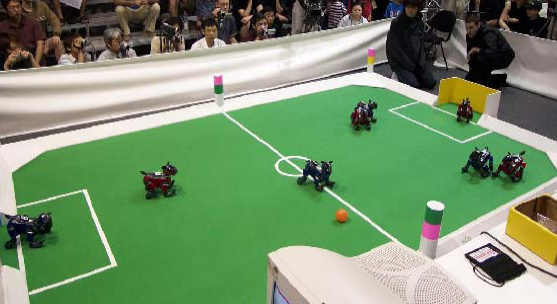
\includegraphics[width=0.5\linewidth]{robot_football}
    \end{center}

\end{frame}

\begin{frame}{Some Kalman Filter facts}

    It is a filter? Not really, it does more than filters do

    \begin{itemize}
        \item Taking into account sensor measurements and process variables.
        \item Prediction forwards (and backwards if needed) in time.
        \item No explicit frequency response
    \end{itemize}

    Kalman Filter is \textbf{recursive}

    \begin{itemize}
        \item It start with initial estimates and continuously updates these
            estimates according to the process model and sensor measurements coming
            in.
    \end{itemize}

    Highly efficient: \textbf{Polynomial in measurement dimensionality} $k$ and
    \textbf{state dimensionality} $n$: $O(k^{2.376} + n^2)$

    \textbf{Optimal}, \ie there is no way of doing better.

\end{frame}

\begin{frame}{Stochasticity}

    \textbf{The true state of a system is unknown}

    \begin{itemize}
        \item We don't know the true speed of an air craft, or the true location
            of the robot.
    \end{itemize}

    This is due to \textbf{stochastic} (= random) noise in the measurements and the
    process.

    \begin{itemize}
        \item Measurement noise example: the air pressure meter reading fluctuates,
            even at the same altitude.
        \item Process noise example: even if we keep the accelerator in the same
            position the car never goes at exactly 60 mph.
    \end{itemize}

\end{frame}

\begin{frame}{Linear system}

A linear equation is a sum of input variables

\begin{itemize}
    \item   For example $f(x)=5x+3$ is linear, $f(x)=cos(x)$ is not.
    \item A linear system can be written in matrix form as $Y=A\cdot X$ or
\end{itemize}

\[
\begin{bmatrix}
    y_1 \\
    \vdots \\ 
    y_n
\end{bmatrix}
=
\begin{bmatrix}
    a_{11} & \cdots & a_{1m}\\ 
    \vdots & \ddots &  \vdots \\ 
    a_{n1} & \cdots & a_{nm}
\end{bmatrix}
\begin{bmatrix}
    x_1 \\
    \vdots \\ 
    x_m
\end{bmatrix}
\]

\end{frame}

\begin{frame}{Normal}

    \href{http://en.wikipedia.org/wiki/Normal_distribution}{Normal} or
    Gaussian

    \begin{itemize}
        \item Symmetrical distribution, captured with two values: \textbf{mean $\mu$ and
            variance $\sigma^2$}.
        \item Described by:

            \[
                \varphi_{\mu, \sigma^2}(x) = \frac{1}{\sqrt{2\pi\sigma^2}\bubblemark{gauss1}} e^{-\frac{(x-\mu)^2}{2 \sigma^2}}
            \]

    \end{itemize}
    \begin{center}
        \resizebox{0.8\linewidth}{!}{
            \begin{tikzpicture}
                \begin{axis}[
                        no markers, domain=-5:5, samples=200,
                    axis lines*=left,
                    every axis y label/.style={at=(current axis.above origin),anchor=south},
                    every axis x label/.style={at=(current axis.right of origin),anchor=west},
                    height=5cm, width=\linewidth,
                    xtick={-5,...,5}, ytick={0.0,0.1,...,1.0},
                    enlargelimits=false, clip=false, axis on top,
                    grid = major
                ]
                    \addplot [very thick,yellow!50!black] {gauss(0,2.24)};
                    \addlegendentry{\tiny$\mu=0, \sigma^2=5.0$};
                    \addplot [very thick,green!50!black] {gauss(-2,0.71)};
                    \addlegendentry{\tiny$\mu=-2, \sigma^2=0.5$};
                    \addplot [very thick,red!50!black] {gauss(0,1)};
                    \addlegendentry{\tiny$\mu=0, \sigma^2=1.0$};
                    \addplot [very thick,blue!50!black] {gauss(0,0.45)};
                    \addlegendentry{\tiny$\mu=0, \sigma^2=0.2$};

                \end{axis}

                \node at (7,1) {\bubblemark{gauss2}};
            \end{tikzpicture}
        }
    \end{center}

    \bubble<1>[190][0.6][1.5cm]{gauss2}{\tiny If these would be measurement distributions of sensors, which sensor is
    the best?}

    \bubble<1>[190][2][2.5cm]{gauss1}{This factor keeps the integral (surface under the curve) equal to 1}

\end{frame}

\begin{frame}{Basic concepts: Gaussian or normal}

    The Kalman Filter assumes that \textbf{measurement and process noise are normal}
    (also known as Gaussian) and \textbf{independent}.

    \vspace{2em}

    \begin{columns}
        \begin{column}{0.4\linewidth}
            \centering
            \only<1>{
                \textbf{Univariate}

            \[
                p\bubblemark[0pt]{prob}(x) \sim \mathcal{N}(\mu, \sigma^2):
            \]

        \[
            p(x) \sim \frac{1}{\sqrt{2\pi\sigma^2}} e^{-\frac{(x-\mu)^2}{2 \sigma^2}}
            \]

        \bubblemark{cov} % dummy one that needs to appear on slides <1>
    }
            \only<2>{
                \textbf{Multivariate}

            \[
                p(x_n) = p(\begin{bmatrix}
                    x_1 \\
                    \vdots \\ 
                    x_n
                \end{bmatrix}) \sim \mathcal{N}_n(\mu, \Sigma\bubblemark[-2ex]{cov}):
            \]

        \[
            p(x_n) =
                \frac{1}{\sqrt{(2\pi)^{n}|\Sigma|}} e^{-\frac{1}{2}(x_n-\mu)^\mathrm{T}\Sigma^{-1}(x_n-\mu)}
            \]
    }
        \end{column}
        \begin{column}{0.6\linewidth}
            \only<1>{
                \begin{tikzpicture}
                    \begin{axis}[
                        anchor=origin,
                        at={(0,0)},
                        no markers, domain=-5:5, samples=200,
                        ytick=\empty,
                        xtick=\empty,
                        axis y line=middle,
                        axis x line=middle,
                        height=5cm, width=\linewidth,
                        ymin=0,ymax=0.5,
                        xmin=-5,xmax=5.3
                    ]
                        \addplot [very thick,black] {gauss(0,1)};

                    \end{axis}

                    \node at (0.8,-0.2) {$\sigma$};
                    \node at (-0.8,-0.2) {$-\sigma$};
                    \node at (0.2,1) {$\mu$};
                    \node at (1,1) {\bubblemark{gauss3}};
                \end{tikzpicture}
                \bubblemark{gauss4}
            }
            \only<2>{
                \centering

                %\pgfplotsset{
                %colormap={whitered}{color(0cm)=(white); color(1cm)=(orange!75!red)}
                %}

            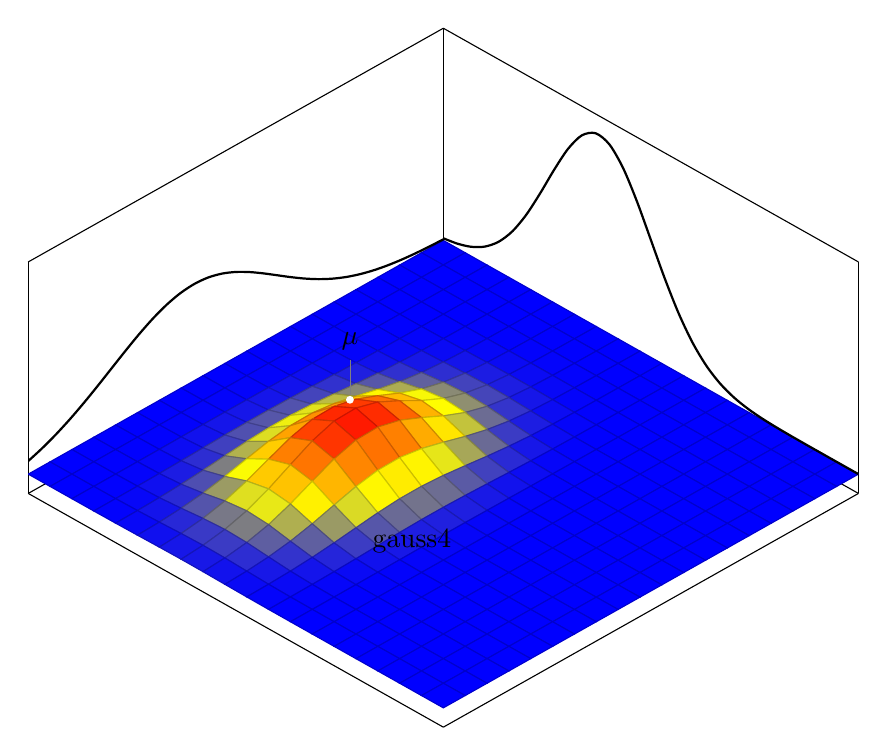
\begin{tikzpicture}[
                    declare function={mu1=0.5;},
                    declare function={mu2=1;},
                    declare function={sigma1=0.5;},
                    declare function={sigma2=1;},
                    declare function={normal(\m,\s)=1/(2*\s*sqrt(pi))*exp(-(x-\m)^2/(2*\s^2));},
                    declare function={bivar(\ma,\sa,\mb,\sb)=1/(2*pi*\sa*\sb) * exp(-((x-\ma)^2/\sa^2 + (y-\mb)^2/\sb^2))/2;}]

            \begin{axis} [
                anchor=origin,
                at={(0,0)},
                width=\linewidth,
                xtick=\empty,
                ytick=\empty,
                ztick=\empty,
                view={45}{55},
                domain=-1:3,
                y domain=-1:4,
            ]
                \addplot3[surf,samples=20] {bivar(mu1,sigma1,mu2,sigma2)};
                \node[circle,inner sep=1pt,fill=white,pin=above:$\mu$] at (axis cs:mu1,mu2,0.2) {};
                \addplot3 [domain=-1:3,samples=31, samples y=0, thick, smooth] (x,4,{normal(mu1,sigma1)});
                \addplot3 [domain=-1:4,samples=31, samples y=0, thick, smooth] (-1,x,{normal(mu2,sigma2)});

            \end{axis}
            \node at (2.5,-0.7) {\bubblemark{gauss4}};
            \end{tikzpicture}

        }
        \end{column}
    \end{columns}

    \bubble<1>[230][1]{gauss3}{For example, a temperature sensor}
    \bubble<1>[100]{prob}{Probability distribution}

    \bubble<2>[120][0.5]{gauss4}{For example, the $x$ and $y$ position of a robot}
    \bubble<2>{cov}{$n \times n$ covariance matrix}

\end{frame}

\begin{frame}{Gaussian function (2)}

    \begin{columns}
        \begin{column}{0.4\linewidth}

            Combining Gaussians ($\mu, \sigma^2$) and ($\nu, r^2$):

            \[
                \mu' = \frac{1}{\sigma^2 + r^2}(r^2\mu + \sigma^2\nu)
            \]
            \[
                \sigma^{2\prime} = \frac{1}{\frac{1}{\sigma^2} + \frac{1}{r^2}}
            \]

            Combining two Gaussians results in a Gaussian that has a \emph{smaller standard deviation}.

        \end{column}
        \begin{column}{0.6\linewidth}

            \begin{tikzpicture}
            \begin{axis}[
            no markers, domain=-5:5, samples=100,
            axis lines*=left,
            every axis y label/.style={at=(current axis.above origin),anchor=south},
            every axis x label/.style={at=(current axis.right of origin),anchor=west},
            height=4.5cm, width=\linewidth,
            xtick={-5,-3,...,5}, ytick={0.0,0.2,...,1.0},
            enlargelimits=false, clip=false, ymax=1.2,
            grid = major
            ]
            \addplot [very thick,green!50!black] {gauss(-2,0.71)};
            \addplot [very thick,red!50!black] {gauss(0,1)};

            \end{axis}

            \end{tikzpicture}

            \begin{tikzpicture}
            \begin{axis}[
            no markers, domain=-5:5, samples=200,
            axis lines*=left,
            every axis y label/.style={at=(current axis.above origin),anchor=south},
            every axis x label/.style={at=(current axis.right of origin),anchor=west},
            height=4.5cm, width=\linewidth,
            xtick={-5,-3,...,5}, ytick={0.0,0.2,...,1.0},
            enlargelimits=false, clip=false, ymax=1.2,
            grid = major
            ]
            \addplot [very thick,green!50!black] {gauss(-2,0.71)};
            \addplot [very thick,red!50!black] {gauss(0,1)};
            \addplot [very thick,cyan!50!black] {gauss(-1.33,.34)};

            \end{axis}

            \end{tikzpicture}

        \end{column}
    \end{columns}

\end{frame}

\begin{frame}{Basic concepts: state}

The \textbf{state} of a process is a vector of real numbers capturing
    the relevant information describing the process. $x = \mathbb{R}^n$

For example

\begin{itemize}
    \item The position and speed of a wheeled robot: $x=[x, y, \theta, \dot{x}, \dot{y}, \dot{\theta}]$
    \item The speed of a missile: $x=[v, t_{thurst}]$
\end{itemize}

\end{frame}

\begin{frame}{The basics}

The Kalman filter needs a number of parameters to run.

These come from the \textbf{process equations}: equations that describe
how the state of the system in the next time step depends on the
current state and any changes that happen to the system.

\pause

For example: a car drives down the road. Its position at time
$t+1$ depends on its position at time $t$, the control input
at $t$ (is the car braking or accelerating) and system dynamics
(it slows down due to friction).

\pause

    Instead of $t$, we use $k$ to denote \emph{discrete time steps}.

\end{frame}

\begin{frame}{The process equations (1)}

    The process is governed by a linear difference equation:

    \vspace{4em}

    \Huge\centering
    $x\bubblemark[-1ex]{pe1}_k = \bubblemark[0pt]{pe2}F \cdot x\bubblemark[-1ex]{pe3}_{k-1} + \bubblemark[0pt]{pe4}B \cdot u\bubblemark[-1ex]{pe5}_{k-1} + \bubblemark[0pt]{pe6}w_{k-1}$

    \bubble<1->[230]{pe1}{The state at time step $k$}
    \bubble<2->[50]{pe2}{$n \times n$ matrix changing the previous state into the current state}
    \bubble<1->[210][1]{pe3}{The state one time step ago}
    \bubble<3->[50]{pe4}{$n \times l$ matrix that maps the control input onto the state}
    \bubble<3->[200][1.5]{pe5}{Control input, a vector of size $l$}
    \bubble<4>[50]{pe6}{The process noise, a vector of size $n$.}

\end{frame}

\begin{frame}{The process equations (2)}

    We take $m$ measurements which will be related to the state
  $x$ according to:

    \vspace{3em}

    \Huge\centering
    $\bubblemark[0pt]{pe7}z_k = H\bubblemark[0pt]{pe8} \cdot x_k + v\bubblemark[0pt]{pe9}_k$

    \bubble<1>[50][0.5][3cm]{pe7}{Measurements, a vector of size $m$}
    \bubble<1>[110][0.5][2.5cm]{pe8}{$m \times n$ matrix mapping the state to the measurements}
    \bubble<1>[130]{pe9}{Measurement noise, a vector of size $m$}

\end{frame}

\begin{frame}{The process equations: recap of main models}

\begin{itemize}
    \item \textbf{State transition model} $F$: matrix $n \times n$ that describes how the state
  changes from $k-1$ to $k$ without controls or noise.
    \item \textbf{Control input model} $B$: matrix $n \times l$ that describes how the
        control $u_{k-1}$ changes the state from $k-1$ to $k$.
    \item \textbf{Observation model} $H$: Matrix $m \times n$ that describes how to map the
  state $x_k$ to the measurements $z_k$.
\end{itemize}

\pause

    \begin{itemize}
        \item \textbf{Process noise model} $w_k$: a vector of size $n$
        \item \textbf{Measurement noise model} $v_k$: a vector of size $m$
    \end{itemize}

\end{frame}

\begin{frame}{Covariance}

    \only<1-2>{
        \href{http://en.wikipedia.org/wiki/Covariance}{Covariance}: measure of how two variables change together.

    Two series $X$ and $Y$ of values, each of size $n$.

    \[
        cov(X,Y) = \overline{(X-\bar{X})(Y-\bar{Y})} = \sum_{i=1}^{n}\frac{(x_i - \bar{X})(y_i - \bar{Y})}{n}
    \]

\only<1>{
    If $cov(X,Y) > 0$, then $X$ and $Y$ tend move together. \\
    If $cov(X,Y) < 0$ then $X$ and $Y$ have an opposite effect on eachother. \\
    And $cov(X,Y) = 0$?

    }
    \only<2>{
        Example: \footnotesize \\
    \begin{align*}
        X &= [4, 2, 3, 4, 5, 5, 3, 1, 1, 2] \\
        Y &= [6, 4, 3, 5, 7, 8, 5, 3, 3, 2] \\
        \bar{X} &= 3 \\
        \bar{Y} &= 4.6 \\
        X - \bar{X} &= [1, -1, 0, 1, 2, 2, 0, -2, -2, -1] \\
        Y - \bar{Y} &= [1.4, -0.6, -1.6, 0.4, 2.4, 3.4, 0.4, -1.6, -1.6, -2.6] \\
        (X-\bar{X})(Y-\bar{Y}) &= [-0.84, 1.56, 2.56, -0.24, 0.96, 1.36, -0.64, 5.76, 5.76, 6.76] \\
        cov(X,Y) &= 2.3 \\
    \end{align*}
}
    }
    \only<3-4>{
        A \href{http://en.wikipedia.org/wiki/Covariance_matrix}{covariance matrix}
    is a matrix showing the covariance of two or more variables to each
    other.

    \begin{itemize}
        \item If one variable changes, does the other variable change as well and in
            what direction?
        \item Example: altitude, temperature and air pressure
    \end{itemize}

    \begin{columns}
        \begin{column}{0.4\linewidth}
            \begin{tabular}{@{}lll@{}}
                \toprule
                altitude & T $^{\circ}C$ & pressure \\ \midrule
                0        & 20          & 1            \\
                1000     & 10          & 0.9          \\
                2000     & 0           & 0.8          \\
                3000     & -10         & 0.7          \\
                4000     & -20         & 0.5          \\
                5000     & -30         & 0.3          \\ \bottomrule
            \end{tabular}

        \end{column}
        \begin{column}{0.6\linewidth}

            \only<4>{
                \begin{tabular}{@{}llll@{}}
                    & \textbf{alt.} & \textbf{T} & \textbf{P} \\
                    \textbf{alt.} & 2916667           & -29166.7      & -400              \\
                    \textbf{T}     & -29166.7          & 291.667      & 4                 \\
                    \textbf{P} & -400              & 4             & 0.057         
                \end{tabular}
            }
        \end{column}
    \end{columns}
}
\end{frame}

\begin{frame}{The process equations (3)}

    The variables $w_k$ and $v_k$ contain the random noise on the state and
    measurements. They (are assumed to) have a \textbf{normal} distribution.

    \vspace{3em}

    \Huge\centering
    $p(w) \sim \mathcal{N}(0, Q)\bubblemark{pe12}$

    $\bubblemark[0pt]{pe10}p(v) \sim \mathcal{N\bubblemark[0pt]{pe11}}(0, R)$

    \bubble<1>[50][0.5][3cm]{pe10}{$p$ means probability distribution}
    \bubble<1>[130][0.5][2.5cm]{pe11}{$\mathcal{N}$ is the notation for a normal distribution}
    \bubble<1>[180]{pe12}{With a \textbf{covariance matrix} of $Q$ and $R$; this reflects the width of the normal distribution}



\end{frame}

\begin{frame}{Round and round goes the Kalman filter}

    \only<1-2>{
        The goal of a Kalman filter is to \textbf{estimate} the state $x$
    at each time step given

    \begin{itemize}
        \item noisy measurements,
        \item control input,
        \item the process equations.
    \end{itemize}

    The state of the filter is represented by two variables:

    \begin{itemize}
        \item $\hat{\mathbf{x}}_{k\mid k}$\bubblemark[-1ex]{aposteriori}: the state estimate at time $k$ given observations up to and including at time $k$
        \item $\mathbf{P}_{k\mid k}$: the \emph{error covariance matrix} (a measure of the estimated accuracy of the state estimate)
    \end{itemize}

    \bubble<2>[200][5.5][4cm]{aposteriori}{the notation $\hat{\mathbf{x}}_{n\mid m}$
    represents the \textbf{estimate} of $\mathbf{x}$ at time $n$ given observations up
    to and including at time $m \leq n$}

    }

    \only<3>{

        The Kalman filter continuously loops through two steps

    \begin{itemize}
        \item The \textbf{state prediction} step.
        \item The \textbf{measurement update} step.
    \end{itemize}

    \centering
    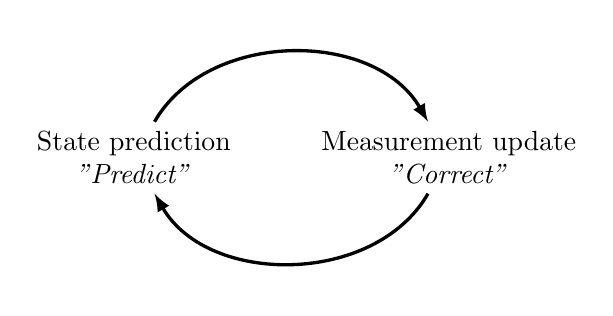
\begin{tikzpicture}[>=latex]

        \node[align=center] at (-2,0) (A) {State prediction\\\emph{"Predict"}};
        \node[align=center] at (2,0) (B) {Measurement update\\\emph{"Correct"}};
        \draw[very thick, ->] (A) to[bend left=60] (B);
        \draw[very thick, ->] (B) to[bend left=60] (A);
    \end{tikzpicture}
    }
    \only<4->{


        The \textbf{Predict} step uses the state estimate from the previous timestep to produce an estimate of the state \textbf{at the current timestep}. This is called the
    \textbf{a priori} estimate

    \begin{itemize}
        \item \emph{A priori} means that the estimate is taken before any new sensor
            measurements have come in.
        \item \textbf{Notation}: $\hat{\mathbf{x}}_{k\mid k-1}$
    \end{itemize}


    }
    \only<5>{

        The \textbf{Correct} step is run after new measurements have come
    in an provide the \textbf{a posteriori} estimate.

    \begin{itemize}
        \item \emph{A posteriori} because the estimate is made after new sensor
            measurements have come in.
        \item \textbf{Notation}: $\hat{\mathbf{x}}_{k\mid k}$
    \end{itemize}
}
\end{frame}

\begin{frame}{Predict step equations}

    \huge\centering
    $\hat{\mathbf{x}}_{k\mid \bubblemark[0pt]{up1}k-1} = \mathbf{F}\cdot \hat{\mathbf{x}}_{k-1\mid \bubblemark[0pt]{up2}k-1} + \mathbf{B}\cdot u_{k-1}$

    \vspace{2em}
    $\mathbf{P}_{k\mid \bubblemark[0pt]{up3}k-1} = \mathbf{F}\cdot \mathbf{P}_{k-1\mid \bubblemark[0pt]{up4}k-1}\cdot \mathbf{F}^{\text{T}} + \mathbf{Q}\bubblemark[0pt]{up5}$


    \bubble<1>[130][0.5][3cm]{up1}{A priori estimate of the state at time $k$}
    \bubble<1>[130][0.5][4cm]{up2}{A posteriori estimate of the state at time $k-1$}
    \bubble<1>[100][0.5][3cm]{up3}{A priori estimate of the error covariance at time $k$}
    \bubble<1>[100][0.5][4cm]{up4}{A poseriori estimate of the error covariance at time $k-1$}
    \bubble<1>[110][0.7][1.5cm]{up5}{Process noise}

\end{frame}


\begin{frame}{Correct step equations (measurement update)}


    \Huge\centering
    $\bubblemark[0pt]{up6}\mathbf{K}_k = \frac{\mathbf{P}_{k\mid k-1}\cdot \mathbf{H}^{\text{T}}}{\mathbf{H}\cdot \mathbf{P}_{k\mid k-1}\cdot \mathbf{H}^{\text{T}} + \bubblemark[0pt]{up8}\mathbf{R}}$

    \vspace{2em}
    \huge
    $\hat{\mathbf{x}}_{k\mid \bubblemark[0pt]{up7}k} = \highlight<2>{\hat{\mathbf{x}}\bubblemark[-1ex]{up10}_{k\mid k-1}} + \highlight<3>{\mathbf{K}_k\cdot (\mathbf{z}_k - \mathbf{H}\bubblemark[-1ex]{up9}\cdot \hat{\mathbf{x}}_{k\mid k-1})}$

    \vspace{2em}
    $\mathbf{P}_{k|k} = (I - \mathbf{K}_k\cdot \mathbf{H})\cdot \mathbf{P}_{k|k-1}$


    \bubble<1>[70][1][4cm]{up6}{The Kalman gain, this needs to calculated first}

    \bubble<1>[130][0.5][3cm]{up7}{The \emph{a posteriori} estimated state}

    \bubble<1>[50][0.5]{up8}{Sensor noise}

    \bubble<3>[270][0.5][5cm]{up9}{(actual measurements - expected measurement) $\times$ Kalman gain}
    \bubble<2>[270][0.5][4cm]{up10}{estimated state at last step}

\end{frame}

\begin{frame}{The Kalman filter loop}

    \centering
    \resizebox{\linewidth}{!}{
    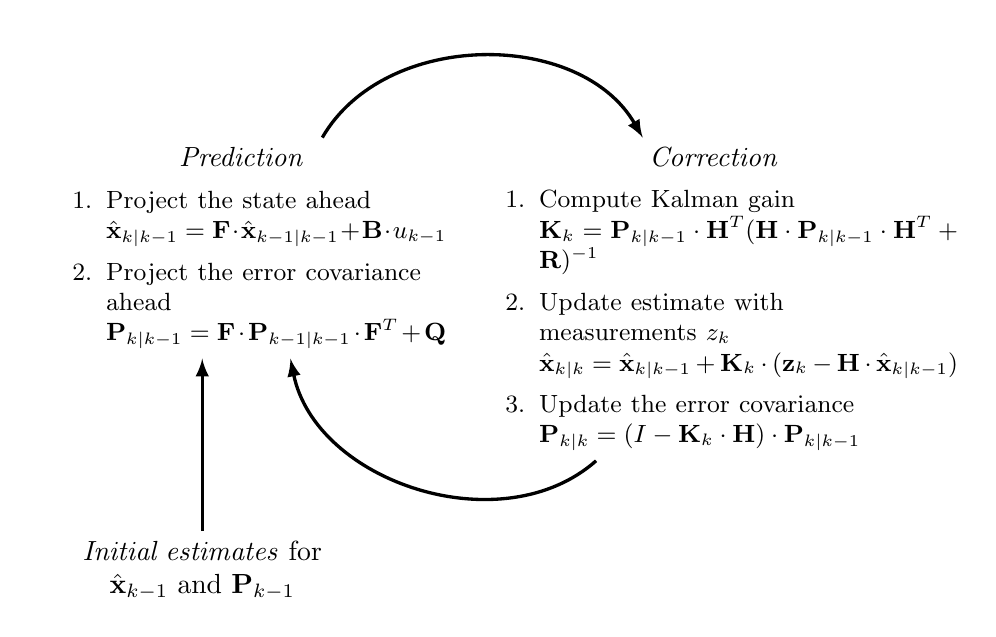
\begin{tikzpicture}[>=latex]

        \node[align=center,text width=5.2cm,anchor=north] at (-3.5,0) (A) {\emph{Prediction}\small
                                                            \begin{enumerate}
                                                                \item Project the state ahead \\
                                                                $\hat{\mathbf{x}}_{k\mid k-1} = \mathbf{F}\cdot \hat{\mathbf{x}}_{k-1\mid k-1} + \mathbf{B}\cdot u_{k-1}$
                                                                \item Project the error covariance ahead \\
                                                                $\mathbf{P}_{k\mid k-1} = \mathbf{F}\cdot \mathbf{P}_{k-1\mid k-1}\cdot \mathbf{F}^{\text{T}} + \mathbf{Q}$
                                                        \end{enumerate}
                                                            };
        \node[align=center,text width=6.2cm,anchor=north] at (2.5,0) (B) {\emph{Correction}\small
                                            \begin{enumerate}
                                                \item Compute Kalman gain \\
                                                $\mathbf{K}_k = \mathbf{P}_{k\mid k-1}\cdot \mathbf{H}^{\text{T}}(\mathbf{H}\cdot \mathbf{P}_{k\mid k-1}\cdot \mathbf{H}^{\text{T}} + \mathbf{R})^{-1}$
                                                \item Update estimate with\\ measurements $z_k$ \\
                                                $\hat{\mathbf{x}}_{k\mid k} = \hat{\mathbf{x}}_{k\mid k-1} + \mathbf{K}_k\cdot (\mathbf{z}_k - \mathbf{H}\cdot \hat{\mathbf{x}}_{k\mid k-1})$
                                                \item Update the error covariance \\
                                                $\mathbf{P}_{k\mid k} = (I - \mathbf{K}_k\cdot \mathbf{H})\cdot \mathbf{P}_{k\mid k-1}$
                                            \end{enumerate}
        };
        \node[align=center,text width=4cm,anchor=north] at (-4,-5) (C) {\emph{Initial estimates} for $\hat{\mathbf{x}}_{k-1}$ and $\mathbf{P}_{k-1}$};

        \draw[very thick, ->] (A) to[bend left=60] (B);
        \draw[very thick, ->] (B) to[bend left=60] (A);
        \draw[very thick, ->] (C) to (C.north |- A.south);
    \end{tikzpicture}
    }

\end{frame}

\begin{frame}{Example 1: measuring a noisy yet constant value}

A Kalman filter to estimate the state of a system with \textbf{one
variable}. For this demonstration, the variable remains
\textbf{constant} (for example, measuring a voltage or a temperature).

    \only<1>{
    \begin{center}
        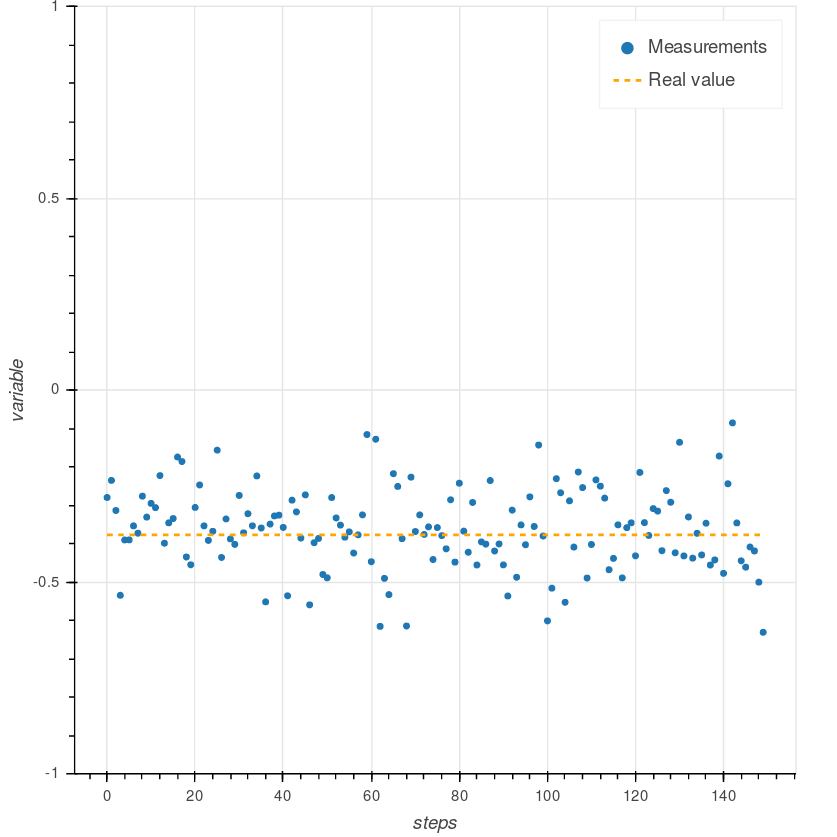
\includegraphics[width=0.5\linewidth]{kalman-ex1-base}
    \end{center}
}

    \only<2-3>{

        \textbf{Prediction}:

    \only<2>{
    \large\centering

    $\hat{\mathbf{x}}_{k\mid k-1} = \mathbf{F}\cdot \hat{\mathbf{x}}_{k-1\mid k-1} + \mathbf{B}\cdot u_{k-1}$

    \vspace{2em}
    $\mathbf{P}_{k\mid k-1} = \mathbf{F}\cdot \mathbf{P}_{k-1\mid k-1}\cdot \mathbf{F}^{\text{T}} + \mathbf{Q}$
    
    }
}

\end{frame}

\begin{frame}[fragile]{Example code}

    \begin{pythoncode}

# Our initial estimate of the system's state
x_estimate_posterior(1) = -0.4;

# The recursive Kalman filter process
for k in range(2,COUNT):
    # Time update phase
    x_estimate_prior(k) = x_estimate_posterior(k-1)
    P_prior(k) = P(k-1) + Q

    # Measurement update phase
    K(k) = P_prior(k) / ( P_prior(k) + R )
    x_estimate_posterior(k) = x_estimate_prior(k) + \
                  K(k) * (z(k) - x_estimate_prior(k))

    P(k) = (1 - K(k)) * P_prior(k)
    \end{pythoncode}

\end{frame}

\imageframe[scale=0.8]{kalman1}

\begin{frame}{Example 2}

  Kalman filter to estimate a moving value (one dimensional).

        \begin{center}
            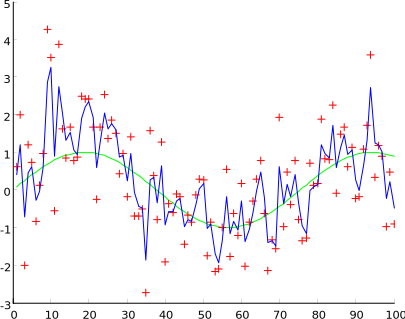
\includegraphics[width=0.7\linewidth]{kalman2}
        \end{center}

\end{frame}

\begin{frame}{Example 3}

  Kalman filter to estimate a moving value, but sensor data becomes
  unreliable

    \begin{columns}
        \begin{column}{0.5\linewidth}
            \begin{center}
                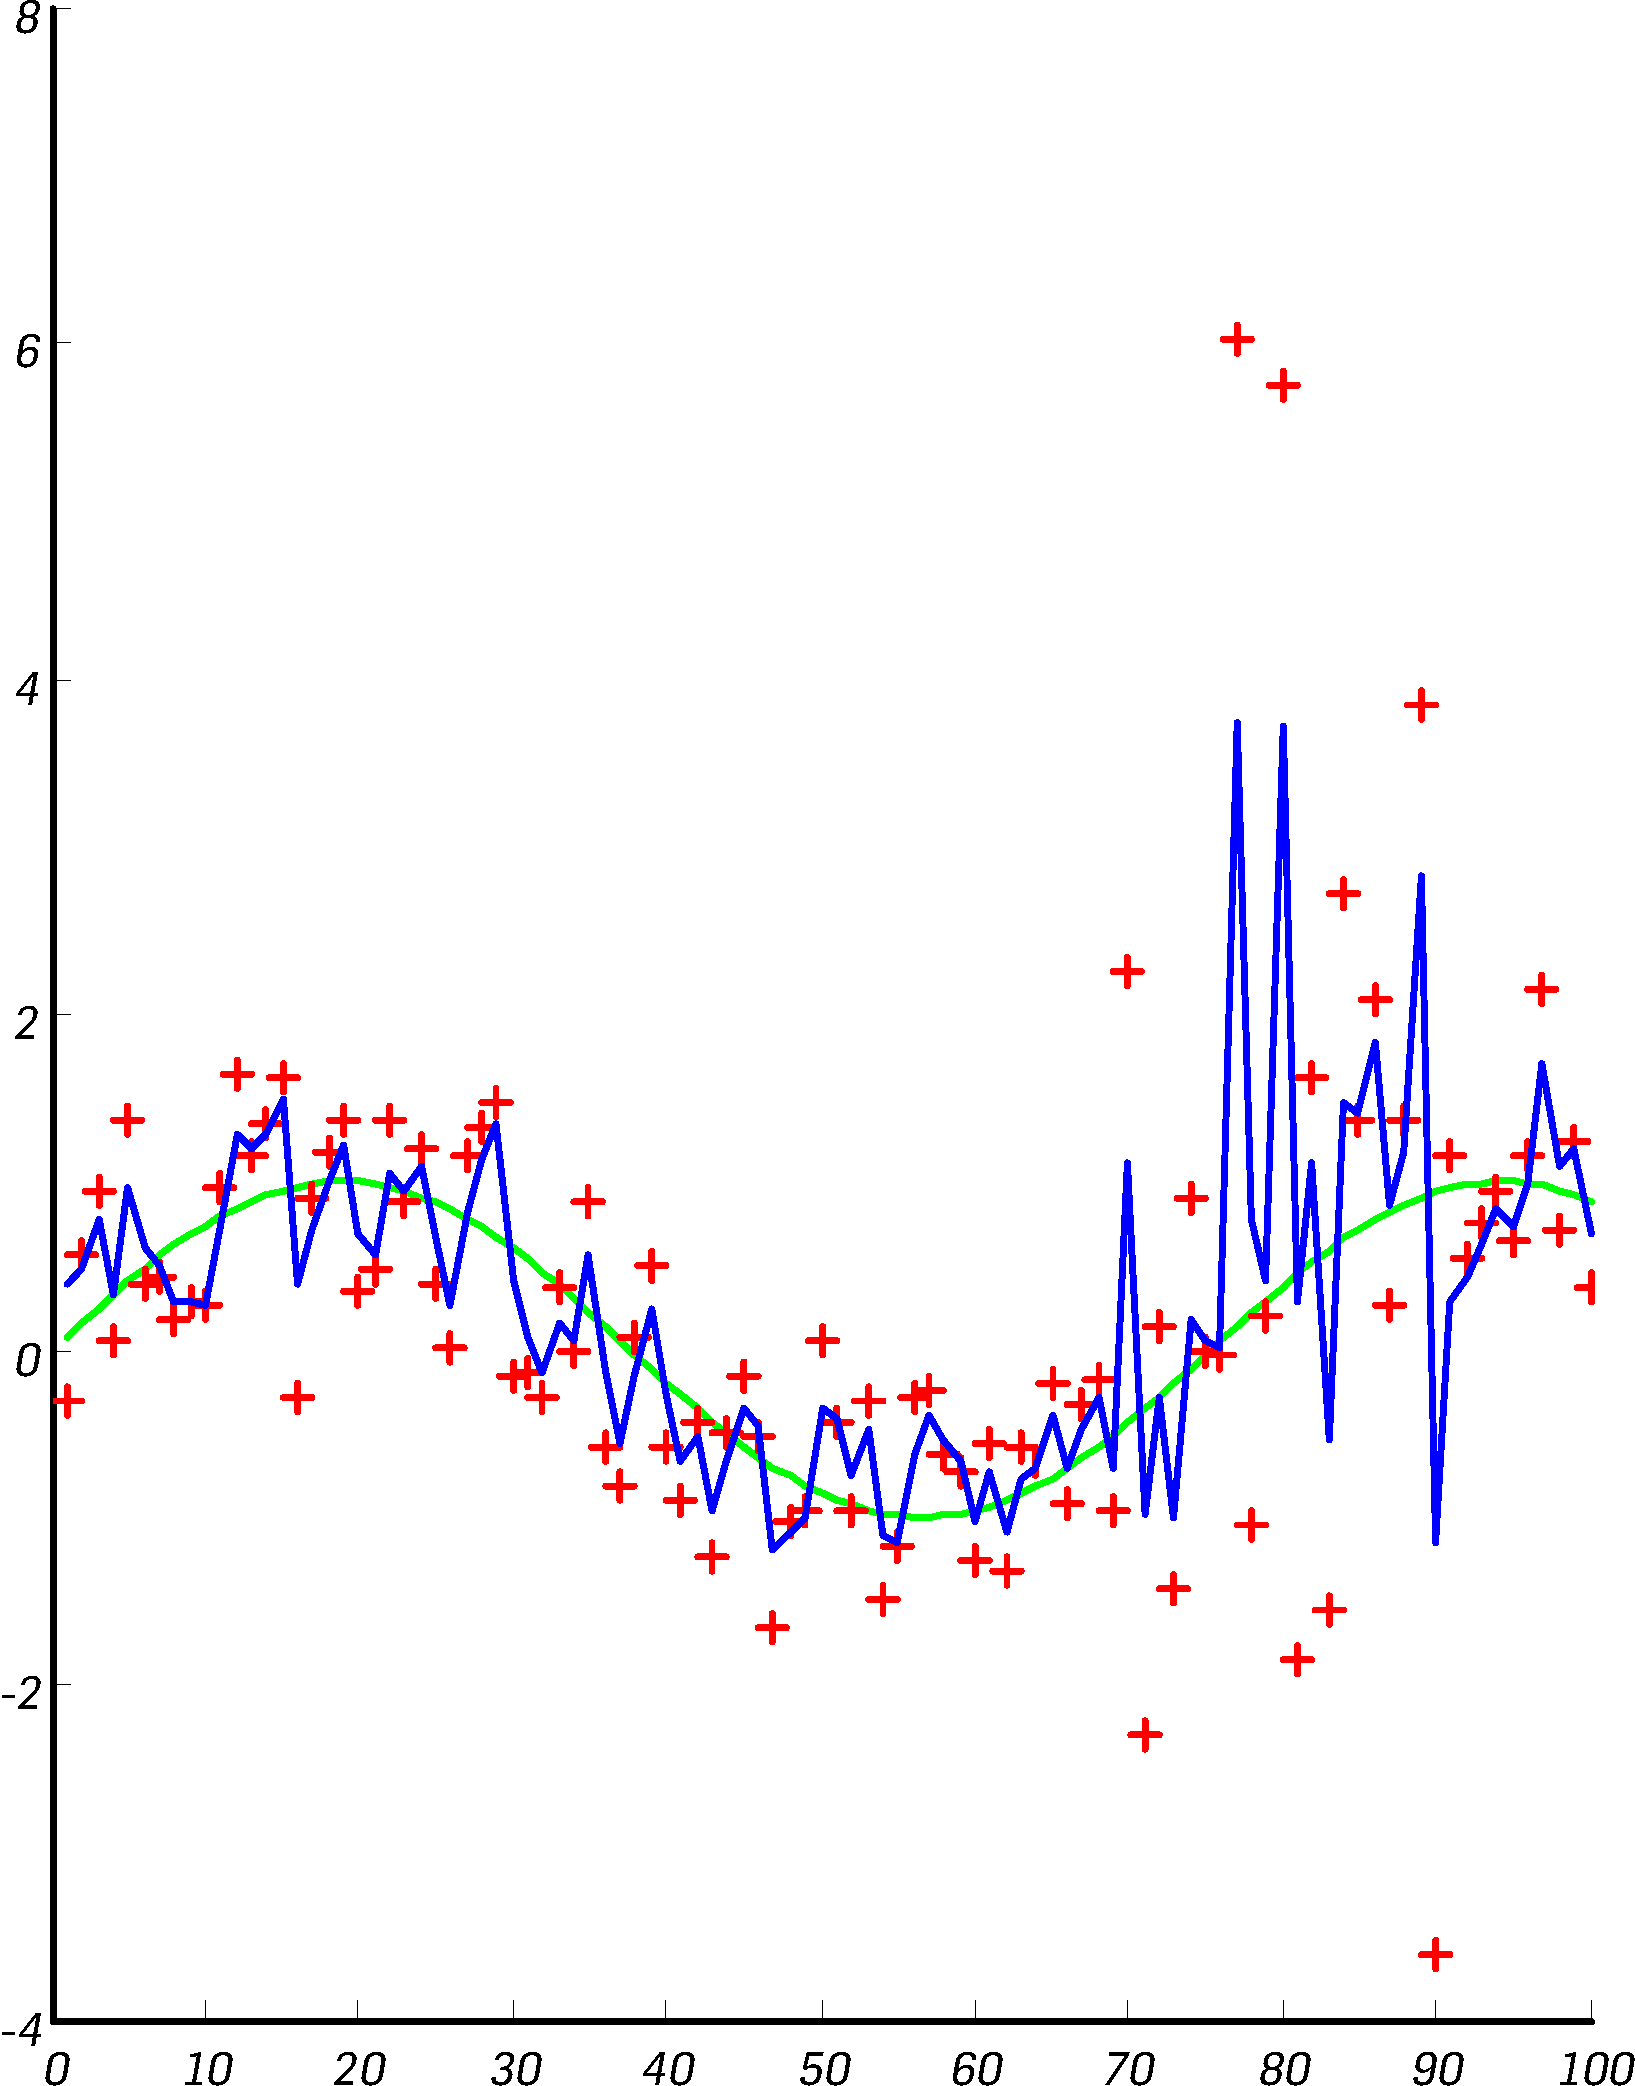
\includegraphics[width=0.8\linewidth]{kalman3}
            \end{center}
        \end{column}
        \begin{column}{0.5\linewidth}
            \begin{center}
                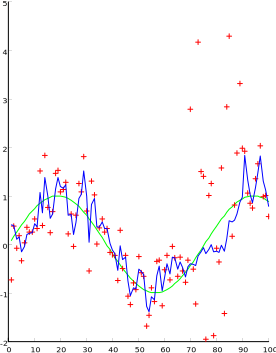
\includegraphics[width=0.8\linewidth]{kalman4}
            \end{center}
        \end{column}
    \end{columns}


Sensor noise shoots up between t = 70 and 90, but KF doesn't know: the Q
matrix is unchanged

Same, but KF is told that sensor noise is high, Q matrix values are
increased

\end{frame}

\begin{frame}{Extension}

In this simple example we only use a state with one variable.

\begin{itemize}
    \item Most systems will have more variables (e.g. pose of a drone has 6
  states).
    \item Most systems will have the first and second derivative in time of all
  variables (i.e. rate of change and acceleration).
\end{itemize}

\end{frame}

\begin{frame}{FAQ}

Is a Kalman Filter similar to \emph{complementary filters}?

\begin{itemize}
    \item Complementary filters are often used to combine accelerometer and gyro
  readings on an IMU.
    \item CF is simple (few lines of code, no matrices) and combines a high and
  low pass filter.
    \item CF does not predict states into the future.
\end{itemize}

What if my problem is non-linear?

\begin{itemize}
    \item There are alternative versions out there such as the Extended Kalman
  Filter (EKF) or Unscented Kalman Filter (UKF).
\end{itemize}

\url{http://www.pieter-jan.com/node/11}

\end{frame}

\begin{frame}{Further reading}

A good text on Kalman filter can be found on

\begin{itemize}
    \item \url{http://www.cs.unc.edu/~welch/media/pdf/kalman_intro.pdf}
\end{itemize}

A good video lecture at Udacity

\begin{itemize}
    \item Lesson 2 of \href{https://www.udacity.com/course/cs373}{Artificial
  Intelligence for Robotics at Udacity}
\end{itemize}

Video demonstrations

Kalman filter on accelerometer and gyro to read stable angle

\begin{itemize}
    \item \url{http://www.youtube.com/watch?v=MJ71V_wxtuU}
    \item \url{http://www.youtube.com/watch?v=Y3TzhXYF0Lg}
\end{itemize}

Kalman filter tracking an airplane

\begin{itemize}
    \item \url{http://www.youtube.com/watch?v=0GSIKwfkFCA}
\end{itemize}

\end{frame}


\begin{frame}{}
    \begin{center}
        \Large
        That's all, folks!\\[2em]
        \normalsize
        Questions:\\
        Portland Square A216 or \url{severin.lemaignan@plymouth.ac.uk} \\[1em]

        Slides:\\ \href{https://github.com/severin-lemaignan/module-mobile-and-humanoid-robots}{\small github.com/severin-lemaignan/module-mobile-and-humanoid-robots}

    \end{center}
\end{frame}



\end{document}
